\documentclass[reprint,amsmath,amssymb,aps,floatfix]{revtex4-1}
%
\usepackage{verbatim}
\usepackage{graphicx}
\usepackage{caption}
\usepackage{dcolumn}
\usepackage{bm}
\usepackage{appendix}
\usepackage{float}
\usepackage{wrapfig}
\usepackage{placeins}
\usepackage{ifthen}
%
\renewcommand{\theequation}{S\arabic{equation}}
\renewcommand{\thefigure}{S\arabic{figure}}
\renewcommand{\thetable}{S\arabic{table}}
\renewcommand{\bibnumfmt}[1]{[S#1]}
\renewcommand{\citenumfont}[1]{S#1}
%
\begin{document}
%
\title{Supplementary Material \\  Weird scaling for 2-D avalanches: \\Curing the faceting, and scaling in the lower critical dimension}
%
\author{L. X. Hayden, Archishman Raju, James P. Sethna}
\affiliation{ LASSP, Physics Department, Cornell University \\
 Ithaca, NY 14853-2501, United States}
%
\date{\today}
\maketitle

\section{\label{app:sims} Simulations}
%
\begin{figure}[!b]
\centering
  	
\includegraphics[scale=0.08]{avalanche_image_size1000000_seed150_r0pt5.png}
  	
\includegraphics[scale=0.08]{avalanche_image_size1000000_seed750_r1pt0.png}
  	\break
  	
\includegraphics[scale=0.08]{avalanche_image_size1000000_seed5050_r5pt0.png}
  	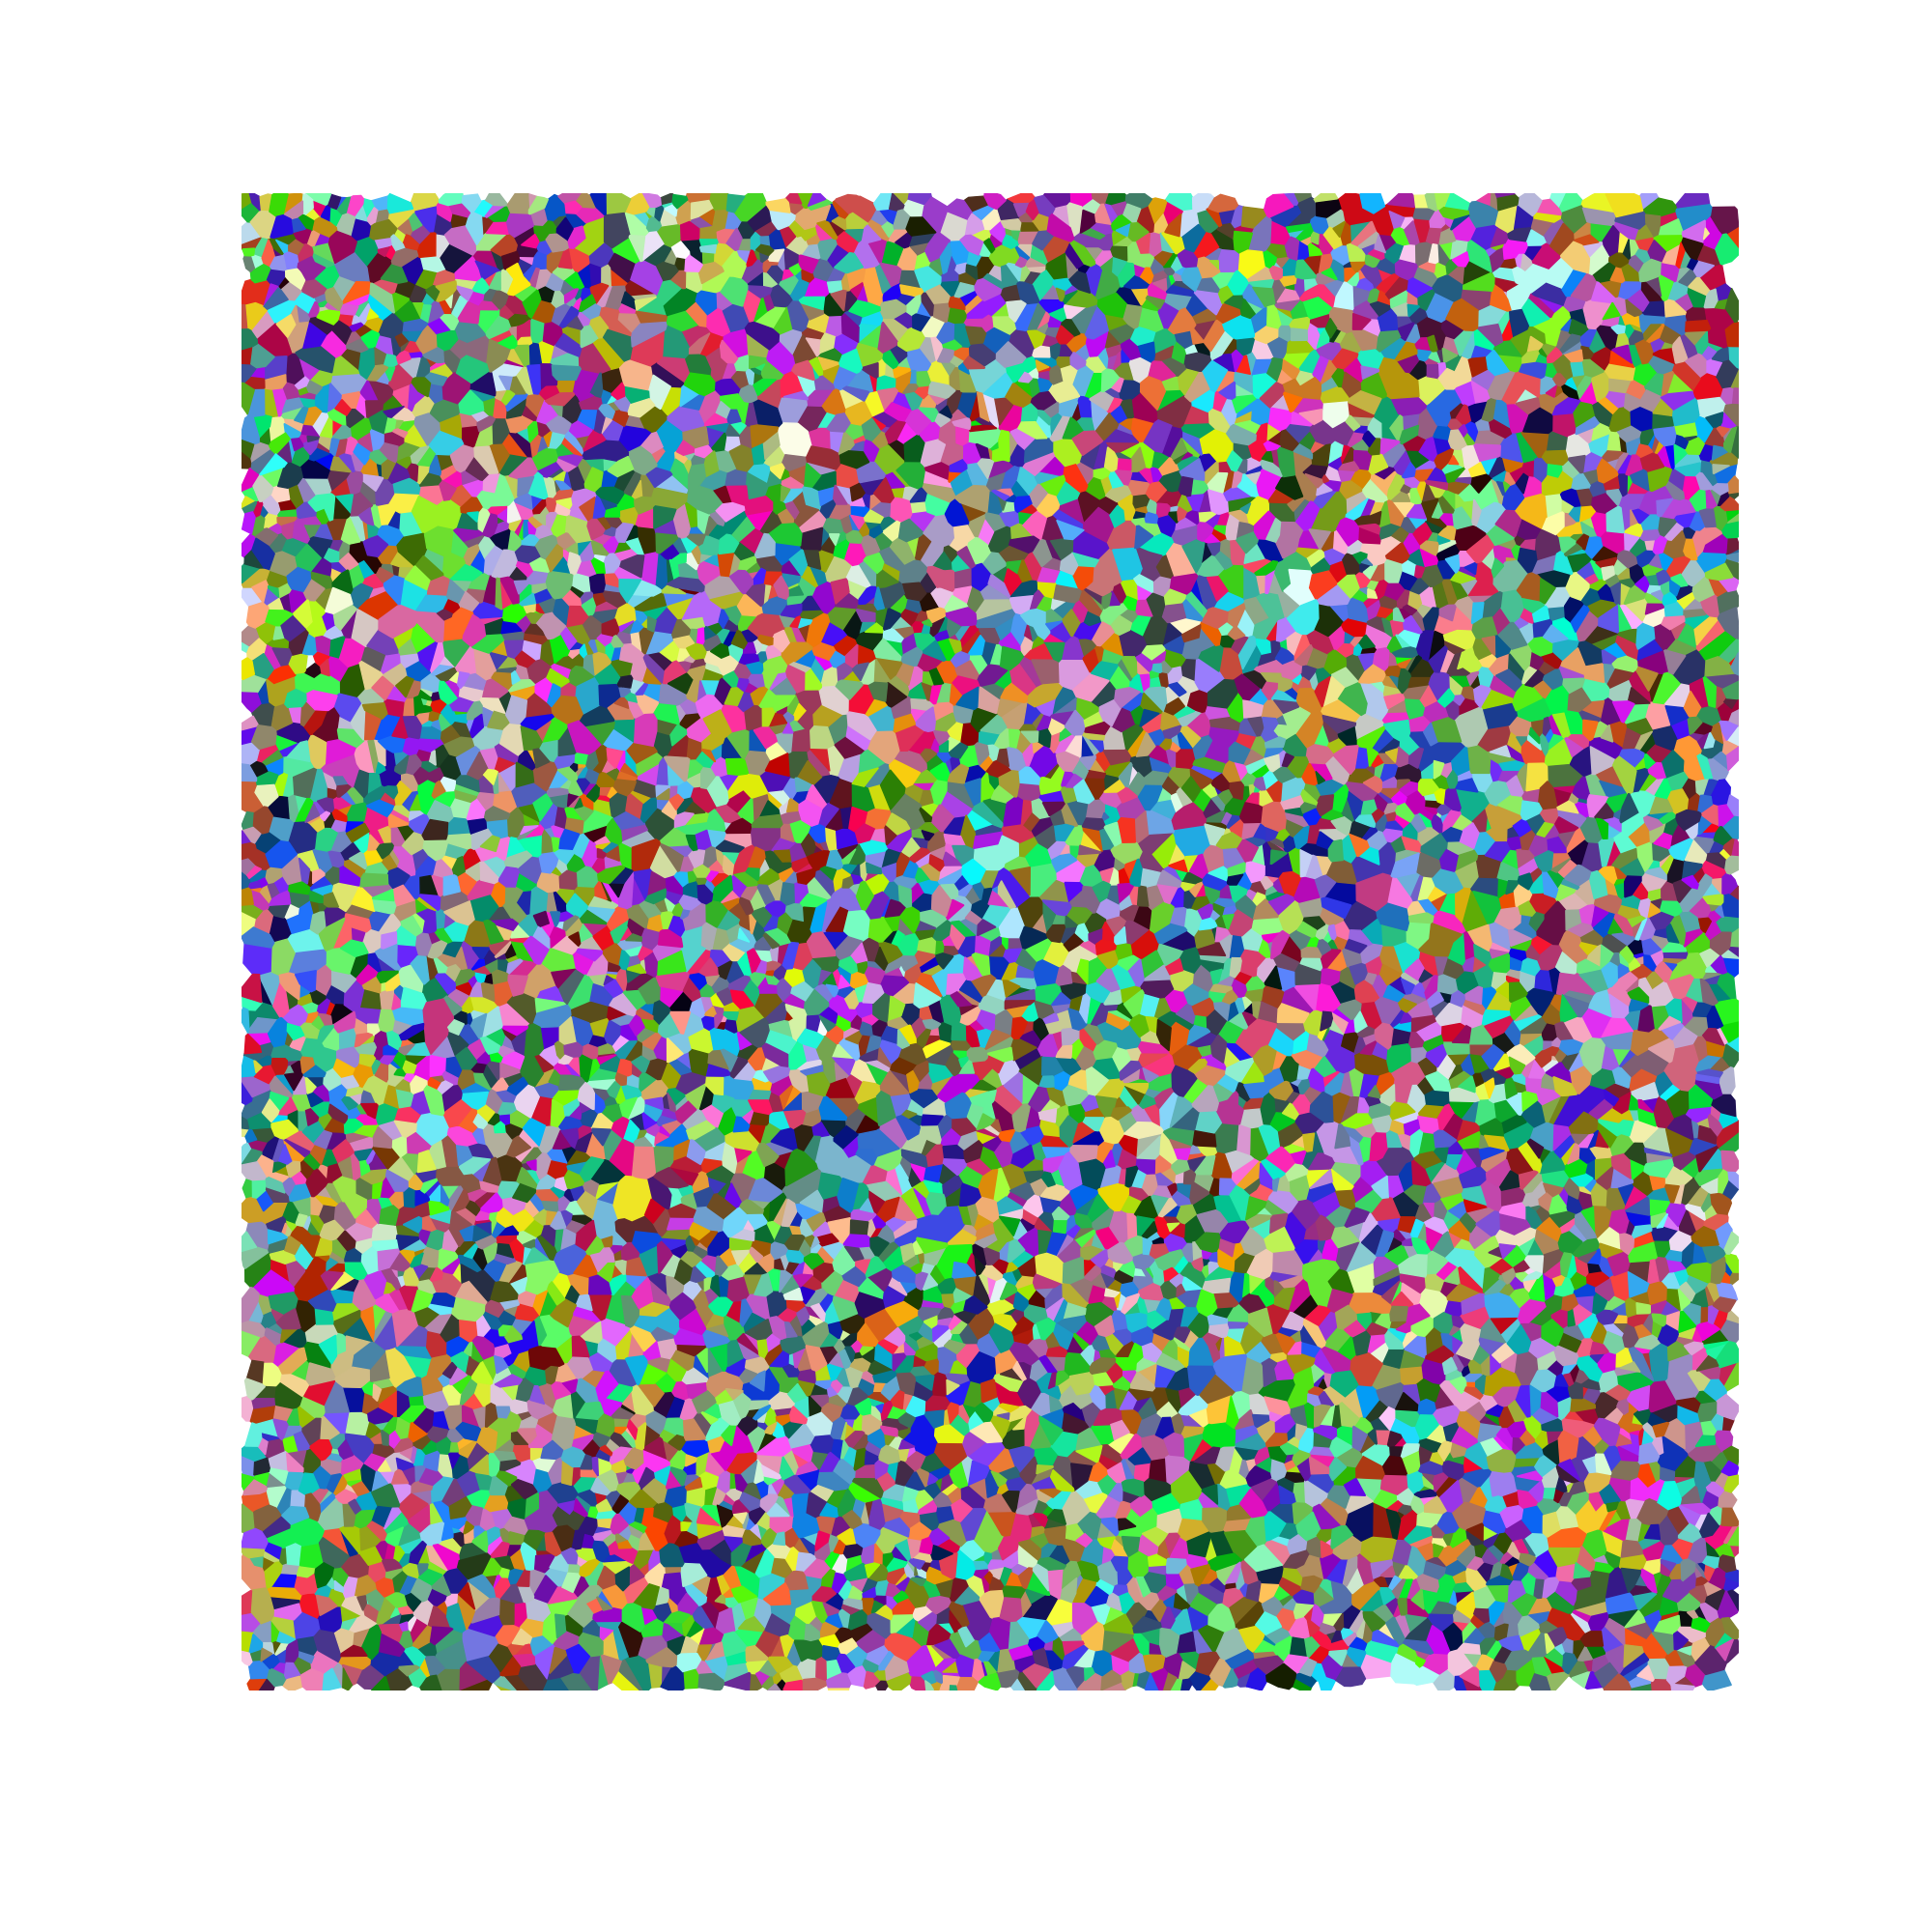
\includegraphics[scale=0.08]{avalanche_image_size1000000_seed50050_r50pt0.png}
  	\captionof{figure}{$r = 0.5,1.0,5.0, 50.0$ from left to right, top to bottom}
  	\label{fig:avalanches}
\end{figure}
%
Experience simulating the RFIM on a square lattice has revealed a propensity for faceting in which the shape of the avalanche size distribution becomes dependent on properties of the lattice for small avalanche sizes.  To mitigate this effect, we perform simulations on a periodic Voronoi lattice where, for each value of $r$, we consider 100 distinct lattices of size 1000x1000.  Voronoi cells were chosen by generating random coordinates between 0 and 1 and constructing the cells with a 2D implementation of Voro++~\cite{Rycroft09} provided by C. H. Rycroft.  Examples of the avalanche behavior for different values of $r$ are shown in Figure \ref{fig:avalanches}. \par
%
We note that much larger simulations have been done on the square lattice, including a thorough analysis of results from a  $131,072^2$ lattice~\cite{Spasojevic11,Spasojevic11-2}. In analysis of in house simulations on a square lattice, however, we encountered long, unnaturally straight avalanche boundaries. We found these distortions strongly affected the shape of the size distribution for small disorders and served to effectively decreased the system size, a difficulty which became dramatically more pronounced as the disorder decreased. In addition to lattice dependent effects infecting the distributions for larger and larger avalanche sizes approaching the critical point, this effective reduction of system size encouraged the use of a Voronoi lattice. \par
%
From the simulations we extract two quantities of interest: the area weighted avalanche size distribution $A(s|r)$~\cite{Chen11} and the change in magnetization of the sample with respect to the field $\frac{dM}{dh}(h|r)$. Alternatively, we may write these as $A(s|w)$ and $\frac{dM}{dh}(h|w)$ where $w$ is a function of $r$ as defined in Appendix~\ref{app:normalform}. 

\section{\label{app:normalform} Normal Form of the RG Disorder Flow}
In the equilibrium model, the flow equation is found to be $dw/d\ell=-(\epsilon/2)w+Aw^3+h.o.t.$ where $\epsilon=D-2$ and $w=r/J$~\cite{BrayMoore85}. For the NE-RFIM, however, $r$ has the symmetry $r \leftrightarrow -r$ while $J$ lacks this symmetry due to the external field. This implies $w \nleftrightarrow -w$ and suggests that the RG flow for $w$ in the NE-RFIM must include a squared order term.\par
%
In principle, there are an infinite series of terms.  Assuming the lower critical dimension $D=2$, we have $\epsilon=0$, and may choose a scale for the disorder $r_s$ such that the prefactor of the squared order term in the flow equation of $w$ is equal to one. Taking $J=1$, the choice we make for $w$ is $w=(r-r_c)/r_s$ where $r_c$ defines the critical disorder. The generic form for the flow equation of $w$ is given by
%
\begin{equation}
	\frac{dw}{d\ell}=w^2+B_1 w^3+ B_2 w^4 + \dots 
\end{equation}
%
\noindent Using only analytic changes of variables, it is possible to remove all terms of $O(4)$ or higher without removing any universal behavior. To demonstrate, consider the change of variables $w = \tilde{w} + b_1\tilde{w}^2+b_2\tilde{w}^3+b_3\tilde{w}^4+\dots$ The resulting flow equation takes the form:
%
\begin{equation}
	\frac{d\tilde{w}}{d\ell}=\tilde{w}^2+B_1 \tilde{w}^3+ (B_1b_2+b_2^2+B_2-b_3) \tilde{w}^4 + \dots
\end{equation} 
%
\noindent With an appropriate choice of $b_2$ in terms of $b_3$, the coefficient of $\tilde{w}^4$ may easily be set to zero. Likewise, all higher order terms may be systematically removed. Dropping the tildes and subscripts for clarity, the final form of the flow equation is given by 
%
\begin{equation}
	\label{eq:TruncNF}
	\frac{dw}{d\ell}=w^2+B w^3
\end{equation}

\section{\label{app:magscale} Scaling Collapse Form for $\frac{dM}{dh}(h|w)$}
The scaling form for the magnetization as a function of field in three dimensions would be 
%
\begin{equation}
	M_{\textrm{3D}}(h|w) \sim w^\beta \mathcal{M}(h-h_c)/w^{\beta\delta})
\end{equation}
%
\noindent yielding a 3D scaling form 
%
\begin{equation}
	\frac{dM_{\textrm{3D}}}{dh}(h|w) =w^{\beta-\beta\delta} \frac{d\mathcal{M}_{\textrm{3D}}}{dh}((h-h_c)/w^{\beta\delta})
\end{equation}
%
\noindent In two dimensions, $w^{\beta\delta}$ is simply replaced by $\eta(w)$ from Eq.~4.\par
%
But what of the term $w^\beta$? It is quite typical for critical exponents to take saturating values in the lower critical dimension. We know that $\beta\delta \to \infty$ as $d\to 2$, but that does not tell us how $\beta$ varies with dimension. Numerical simulations in higher dimensions~\cite{Perkovic96} show $\beta$ decreasing from its mean-field value $\beta_{\textrm{MF}}=1/2$ in $d=6$ down to $\beta_{\textrm{3D}} = 0.035 \pm 0.0280$ in three dimensions. It is natural to expect that $\beta = 0$ in two dimensions, and that the universal scaling function $\mathcal{M}$ varies from $-1$ to $1$ as the field increases (saturating the behavior). This implies that
%
\begin{equation}
	\frac{dM}{dh}(h|w)=\eta(w)^{-1}\frac{d\mathcal{M}}{dh}(v)
\end{equation}
%
\noindent where the invariant scaling combination
%
\begin{equation}
	v = (h-h_{\textrm{max}})/\eta(w).
\end{equation}
%
\noindent It is traditional to scale with $h-h_c$, but since $h_{\textrm{max}}-h_c\propto \eta(w)$, scaling to $h_{\textrm{max}}$ is equivalent. The form chosen for the universal scaling function $\frac{d\mathcal{M}}{dh}(h|w)$ is given in Appendix~\ref{app:universal}.


\section{\label{app:correlation} Correlation Length}
The correlation length may be calculated directly from the flow equation of the disorder. For the transcritical form
%
\begin{equation}
	\frac{dw}{d\ell} = w^2+B w^3
\end{equation}
%
\noindent we have
%
\begin{equation}
	\int_{\ell_0}^{\ell^*}d\ell = \int_{w_0}^{w^*}\frac{dw}{w^2+B w^3}
\end{equation}
%
\noindent where $(w_0,\ell_0)$ denotes an initial point and $(w^*, \ell^*)$ a fixed point of the RG, a constant. Performing the integration and letting $(w_0,\ell_0)\rightarrow(w,\ell)$ we obtain
%
\begin{equation}
	\ell \sim B\log\bigg{(}B+\frac{1}{w}\bigg{)}-\frac{1}{w}
\end{equation}
%
\noindent We have
%
\begin{equation}
	\xi\sim \exp(-\ell)
\end{equation}
%
\noindent hence
%
\begin{equation}
	\xi\sim\bigg{(}\frac{1}{w}+B\bigg{)}^{-B}\exp\bigg{(}\frac{1}{w}\bigg{)}
\end{equation}


\section{\label{app:invariant} Invariant Scaling Combinations}
\subsection{\label{app:powerlaw} Power Law Form}
%
As our invariant parameter combinations are unorthodox, we provide here a thorough derivation and a comparison to the usual power law `homogeneous' variables seen at the usual hyperbolic fixed points. The invariant scaling combinations corresponding to traditional power law scaling may be simply derived from the flow equations in 3 and higher dimensions. We have
%
\begin{equation}
	\begin{split}
		\frac{dw}{d\ell}&=\frac{1}{\nu} w\\
		\frac{ds}{d\ell}&=- \frac{1}{\sigma\nu}s\\
		\frac{dh}{d\ell}&=\frac{\beta\delta}{\nu}h
	\end{split}
\end{equation}
%
\noindent Taking $(dw/d\ell)/(ds/d\ell)$ and integrating gives
%
\begin{equation}
	\int_{w_0}^{w^*}\frac{dw}{(1/\nu) w} = \int_{s_0}^{s^*}\frac{ds}{(-1/\sigma\nu) s} 
\end{equation}
%
\noindent Performing the integral and working through the algebra
%
\begin{equation}
	\begin{split}
		&\log\ w^*-\log\ w_0 = -\sigma(\log\ s^*-\log\ s_0)\\
		&\Rightarrow  \sigma \log(s_0)+ \log\ w_0= \sigma \log\ s^*+\log\ w^*\\
		&\Rightarrow s_0^\sigma w_0=\textrm{constant}
	\end{split}
\end{equation}
%
\noindent where $(w^*, s^*)$ corresponds to the fixed point of the RG and is hence a constant. The invariant scaling combination in this instance is thus
%
\begin{equation}
	s^\sigma w
\end{equation}
%
which agrees with the results in 3 and higher dimensions~\cite{Perkovic96}. Similarly for $h$ we have
%
\begin{equation}
	\int_{w_0}^{w^*}\frac{dw}{(1/\nu) w} = \int_{h_0}^{h^*}\frac{dh}{(\beta\delta/\nu) h} 
\end{equation}
%
\noindent Performing the integral and working through the algebra
%
\begin{equation}
	\begin{split}
		&\beta\delta(\log\ w^*-\log\ w_0) = \log\ h^*-\log\ h_0\\
		&\Rightarrow  \log\ h_0 - \beta\delta \log\ w_0= \log\ h^*- \beta\delta \log\ w^*\\
		&\Rightarrow h_0 w_0^{-\beta\delta}=\textrm{constant}
	\end{split}
\end{equation}
%
\noindent The invariant scaling combination is hence
%
\begin{equation}
	h/ w^{\beta\delta}
\end{equation}
%
\noindent which again agrees with the literature~\cite{Perkovic96}.
%
\subsection{\label{app:truncated} Transcritical Form}
The flow equations using the transcritical form for the disorder are as follows
%
\begin{equation}
	\begin{split}
		&\frac{dw}{d\ell}= w^2+B w^3\\
		&\frac{ds}{d\ell}= -d_f s-C s w\\
		&\frac{dh}{d\ell}= \lambda_h h+F h w
		\end{split}
\end{equation}
%
As before, we take the integral of $dw/d\ell$ over $ds/d\ell$ and obtain
%
\begin{equation}
	\int_{s_0}^{s^*}(1/s)\ ds = \int_{w_0}^{w^*}\frac{-d_f-Cw}{w^2+ B w^3}\ dw
\end{equation}
%
\noindent Solving for $s_0$ we have
%
\begin{equation}
	s_0 = \bigg{(}B+\frac{1}{w_0}\bigg{)}^{-B d_f+C}\exp \bigg{(}\frac{d_f}{w_0}\bigg{)}f(w^*, s^*)
\end{equation} 
%
\noindent where $f(w^*, s^*)$ denotes a function of $w^*$ and $s^*$ and is therefore constant. The invariant scaling combination in this case is then
%
\begin{equation}
	\frac{s}{\Sigma_{\textrm{th}}(w)}
\end{equation}
%
\noindent where
%
\begin{equation}
	\Sigma_{\textrm{th}}(w) = \bigg{(}B+\frac{1}{w}\bigg{)}^{-B d_f+C}\exp \bigg{(}\frac{d_f}{w}\bigg{)}
\end{equation}
%
\noindent Likewise for $h$ we obtain an invariant scaling combination
%
\begin{equation}
	\frac{h}{\eta_{\textrm{th}}(w)}
\end{equation}
%
\noindent where
%
\begin{equation}
	\eta_{\textrm{th}}(w) = \bigg{(}B+\frac{1}{w}\bigg{)}^{B \lambda_h-F}\exp \bigg{(}-\frac{\lambda_h}{w}\bigg{)}
\end{equation}
%
\subsection{\label{app:well-behaved} Alternative Transcritical Form}
Applying our methods to the 2D equilibrium NE-RFIM, we find that the fixed point is given by a pitchfork bifurcation corresponding to
%
\begin{equation}
\frac{dw}{d\ell}= w^3-D w^5
\end{equation} 
%
In this instance, however, the behavior of the correlation length suggests an alternative choice for the normal form 
%
\begin{equation}
\frac{dw}{d\ell}= \frac{w^3}{1+D w^2}
\end{equation}
% 
as discussed in ~\cite{Raju17}. This form, while retaining the pitchfork behavior, produces a well behaved correlation function that is also able to capture higher order corrections to scaling which we expect to become important further from the critical point. We may apply the same procedure in the non-equilibrium case, although the function for the correlation length here appears well behaved. This yields an alternative form for the transcritical bifurcation given by
%
\begin{equation}
	\begin{split}
		&\frac{dw}{d\ell}= \frac{w^2}{1-B w}\\
		&\frac{ds}{d\ell}= -d_f s-C s w\\
		&\frac{dh}{d\ell}= \lambda_h h+F h w
		\end{split}
\end{equation}
%
As before, to determine $\Sigma(w)$, we take the integral of $dw/d\ell$ over $ds/d\ell$ and obtain
%
\begin{equation}
	\int_{s_0}^{s^*}(1/s)\ ds = \int_{w_0}^{w^*}\frac{-d_f-Cw}{w^2/(1- B w)}\ dw
\end{equation}
%
\noindent Solving for $s_0$ we have
%
\begin{equation}
	s_0 =w_0^{B d_f -C} \exp \bigg{(}\frac{d_f}{w_0}+B C w_0\bigg{)}f(w^*, s^*)
\end{equation} 
%
\noindent where $f(w^*, s^*)$ denotes a function of $w^*$ and $s^*$ and is therefore constant. The invariant scaling combination in this case is then
%
\begin{equation}
	\frac{s}{\Sigma_{\textrm{alt}}(w)}
\end{equation}
%
\noindent where
%
\begin{equation}
	\Sigma_{\textrm{alt}}(w) = w^{B d_f -C}\exp \bigg{(}\frac{d_f}{w}+B C w\bigg{)}
\end{equation}
%
\noindent Likewise for $h$ we obtain an invariant scaling combination
%
\begin{equation}
	\frac{h}{\eta_{\textrm{alt}}(w)}
\end{equation}
%
\noindent where
%
\begin{equation}
	\eta_{\textrm{alt}}(w) = w^{-B \lambda_h + F}\exp \bigg{(}-\frac{\lambda_h}{w}-B F w\bigg{)}
\end{equation}
%
\subsection{\label{app:pitchfork} Pitchfork Form}
The flow equations using a pitchfork form for the disorder are as follows
%
\begin{equation}
	\begin{split}
		&\frac{dw}{d\ell}= w^3+B w^5\\
		&\frac{ds}{d\ell}= -d_f s-C s w\\
		&\frac{dh}{d\ell}= \lambda_h h+F h w
		\end{split}
\end{equation}
%
As before, we take the integral of $dw/d\ell$ over $ds/d\ell$ and obtain
%
\begin{equation}
	\int_{s_0}^{s^*}(1/s)\ ds = \int_{w_0}^{w^*}\frac{-d_f-Cw}{w^3+B w^5}\ dw
\end{equation}
%
\noindent Solving for $s_0$ we have
%
\begin{equation}
	\begin{split}
		s_0 \sim &w_0^{B d_f}(1+B w_0^2)^{-\frac{B d_f}{2}} \\
		&\times \exp \bigg{(}\frac{d_f}{2w_0^2}+\frac{C}{w_0}+\sqrt{B} C \arctan(\sqrt{B}w_0)\bigg{)}
	\end{split}
\end{equation} 
%
\noindent The invariant scaling combination in this case is then
%
\begin{equation}
	\frac{s}{\Sigma_{\textrm{pf}}(w)}
\end{equation}
%
\noindent where
%
\begin{equation}
	\begin{split}
		\Sigma_{\textrm{pf}}(w)  = & w^{B d_f}(1+B w^2)^{-\frac{B d_f}{2}} \\
		& \times \exp \bigg{(}\frac{d_f}{2w^2}+\frac{C}{w}+\sqrt{B} C \arctan(\sqrt{B}w)\bigg{)}
	\end{split}
\end{equation}
%
\noindent Likewise for $h$ we obtain an invariant scaling combination
%
\begin{equation}
	\frac{h}{\eta_{\textrm{pf}}(w)}
\end{equation}
%
\noindent where
%
\begin{equation}
	\begin{split}
		\eta_{\textrm{pf}}(w) = & w^{-B \lambda_h}(1+B w^2)^{\frac{B \lambda_h}{2}} \\
		&\times \exp \bigg{(}-\frac{\lambda_h}{2w^2}-\frac{F}{w}-\sqrt{B} F \arctan(\sqrt{B}w)\bigg{)}
	\end{split}
\end{equation}

\section{\label{app:universal} Universal Scaling Function Forms}
In order to perform our fits, we choose functional forms for the universal scaling functions. For the area weighted avalanche size distribution, we choose 
%
\begin{equation}
	\label{eqn:univA}
	\mathcal{A}(v_s) = \frac{1}{\mathcal{A}_N}v_s^a\exp(v_s^b)
\end{equation}
%
\noindent where the leading power law $v_s^x$ has been absorbed into $v_s^a$ here and $\mathcal{A}_N$ is the normalization factor $\mathcal{A}_N = \big{[}\Gamma\big{(}\frac{a}{b}\big{)}\gamma\big{(}\frac{a}{b}, \Sigma(w)^{-2b}\big{)}\big{]}/b$ where $\gamma$ denotes the regularized upper incomplete gamma function. \par
%
For $d\mathcal{M}/dh$ we choose
%
\begin{equation}
	\frac{d\mathcal{M}}{dh}(v_h)=   \frac{1}{\frac{d\mathcal{M}}{dh}_{N}} \exp\bigg{[}\bigg{(}\frac{-v_h^2}{a+b v_h+c v_h^2}\bigg{)}^{d/2}\bigg{]}
\end{equation}
%
\noindent where $\frac{d\mathcal{M}}{dh}_{N}$ is a normalization factor computed as a sum of $\frac{dM}{dh}$ over the data range. 

\section{\label{app:compare} Form Comparison}
In the lower critical dimension, we expect the fixed point to be governed by a transcritical bifurcation. Assuming compact avalanches, this yields directly
%
\begin{equation}
	\Sigma_{\textrm{th}}(w) = \Sigma_s\bigg{(}B+\frac{1}{w}\bigg{)}^{-B d_f}\exp \bigg{(}\frac{d_f}{w}\bigg{)}
\end{equation}
%
\noindent where $\Sigma_s$ is an unknown scale factor. We may compare this functional form for $\Sigma$ with that derived assuming power law scaling and one assuming a pitchfork bifurcation as appears in the equilibrium model. For the power law case we have the invariant scaling combination
%
\begin{equation}
	s^\sigma w
\end{equation}
%
\noindent which is equilvalent to 
%
\begin{equation}
	s/w^{-1/\sigma}
\end{equation}
%
\noindent such that $\Sigma_{\textrm{pl}}(w)$ for the power law case would be given by:
%
\begin{equation}
	\Sigma_{\textrm{pl}}(w)=\Sigma_s'w^{-1/\sigma}
\end{equation}
%
\noindent where $\Sigma_s'$ is an unknown scale factor determined by fitting to a power law form. For the pitchfork case we have from Appendix~\ref{app:pitchfork}
%
\begin{equation}
	\begin{split}
		\Sigma_{\textrm{pf}}(w) = &\Sigma_s'' w^{B d_f}(1+B w^2)^{-\frac{B d_f}{2}} \\ 
		&\times\exp \bigg{(}\frac{d_f}{2w^2}+\frac{C}{w}+\sqrt{B} C \arctan(\sqrt{B}w)\bigg{)}
	\end{split}
\end{equation}
%
\noindent where $\Sigma_s''$ is the unknown scale factor. We have that $w=(r-r_c)/r_s$ for each of the functional forms considered. The comparison of the fits are shown in Figure~3. 

\section{\label{app:goodfits} Parameter Values}
The parameter values corresponding to resonable fits are highly variable. For example, we may restrict $\lambda_h=1$ corresponding to the Harris criteria for this model~\cite{Perkovic96} and still obtain an acceptable fit.  A wide range of fits with various restrictions are shown in Figures~\ref{fig:Sigmatruncated}, ~\ref{fig:etatruncated}, ~\ref{fig:Sigmawellbehaved}, and~\ref{fig:etawellbehaved}. Corresponding best fit parameter values are shown in Tables~\ref{tab:truncatedcompare} and~\ref{tab:wellbehavedcompare}. As anticipated, the alternative form for the transcritical bifurcation is able to better capture the behavior far from the critical point.
%
\begin{figure}
	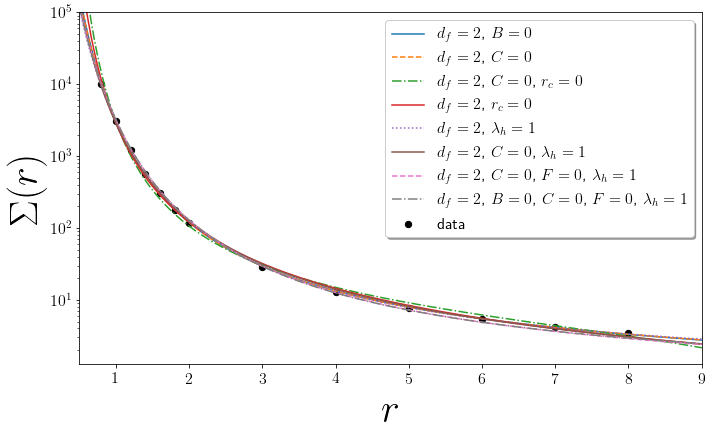
\includegraphics[width=0.5\textwidth]{Sigma_truncated_comparison.png}
	\caption{Fit comparisons $\Sigma_{\textrm{th}}(w)$, transcritical form}	
	\label{fig:Sigmatruncated}
\end{figure}
%
\begin{figure}
	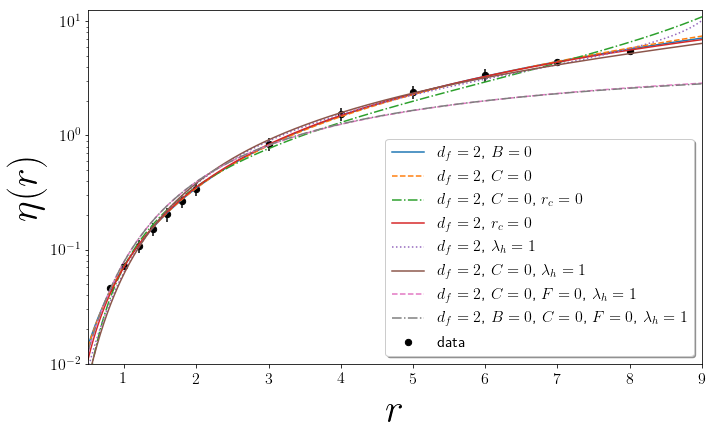
\includegraphics[width=0.5\textwidth]{eta_truncated_comparison.png}
	\caption{Fit comparisons $\eta_{\textrm{th}}(w)$, transcritical form}
	\label{fig:etatruncated}
\end{figure}
%
\begin{table*}
	\begin{tabular}{|c|c|c|c|c|c|c|c|c|}
		\hline
		$r_s$ & $5.11 \pm 0.54$ & $5.49 \pm 0.18$ & $2.91 \pm 0.27$ & $2.04 \pm 0.34$&  $6.89 \pm 0.63$ & $4.93 \pm 0.15$ & $6.78 \pm 0.20$ & $7.40 \pm 0.12$ \\
		$r_c$ & $-0.42 \pm 0.11$ & $-0.46 \pm 0.06$ & \textbf{0} & \textbf{0}&  $-0.65 \pm 0.10$ & $4.93 \pm 0.15$ & $-0.64 \pm 0.06$ & $-0.70 \pm 0.03$ \\
		$\Sigma_s$ & $1.24 \pm 0.66$ & $1.11 \pm 0.05$ & $5.27 \pm 1.96$ & $14.40 \pm 8.84$&  $0.68 \pm 0.22$ & $1.64 \pm 0.04$ & $0.64 \pm 0.04$ & $0.54 \pm 0.005$ \\
		$\eta_s$ & $3.16 \pm 0.11$ & $3.11 \pm 0.44$ & $1.02 \pm 0.52$ & $0.50 \pm 0.41$&  $6.26 \pm 0.25$ & $4.33 \pm 0.42$ & $5.55 \pm 0.52$ & $6.08 \pm 0.82$ \\
		$d_f$ & \textbf{2} & \textbf{2} & \textbf{2} & \textbf{2}& \textbf{2} & \textbf{2} & \textbf{2} & \textbf{2}\\
		$\lambda_h$ & $0.44 \pm 0.04$ & $0.52 \pm 0.07$ & $0.61 \pm 0.05$ & $0.24 \pm 0.08$& \textbf{1} & \textbf{1} & \textbf{1} & \textbf{1} \\
		$B$ & \textbf{0} & $-0.15 \pm 0.01$ & $-0.27 \pm 0.03$ & $0.039 \pm 0.007$ & $ -0.69 \pm 0.21$ & $-0.25 \pm 0.03$ & $-0.09 \pm 0.01$ & \textbf{0} \\
		$C$ & $0.46 \pm 0.10$ & \textbf{0} & \textbf{0} & $1.76 \pm 0.28$ &  $-1.38 \pm 0.52$ & \textbf{0} & \textbf{0} & \textbf{0} \\
		$F$ & $1.72 \pm 0.08$ & $1.33 \pm 0.12$ & $0.73 \pm 0.02$ & $2.02 \pm 0.13$&  $-0.37 \pm 0.35$ & $0.45 \pm 0.06$ & \textbf{0} & \textbf{0} \\
		\hline
	\end{tabular}
	\caption{	\label{tab:truncatedcompare} Table of the best fit values corresponding to Figures~\ref{fig:Sigmatruncated} and~\ref{fig:etatruncated}. Values in bold correspond to values fixed in the fit.}
\end{table*}
%
\begin{figure}
	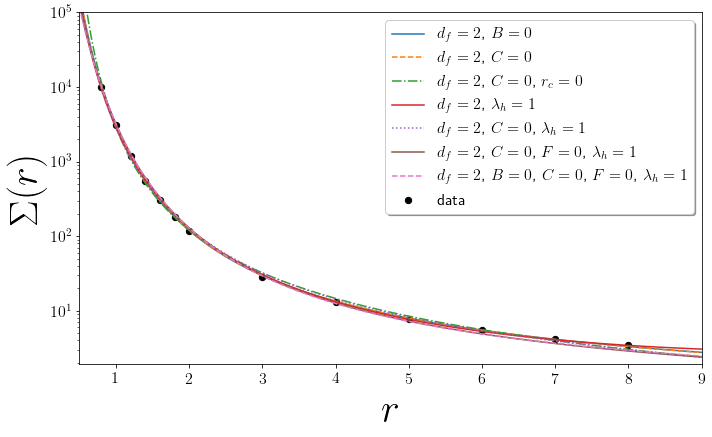
\includegraphics[width=0.5\textwidth]{Sigma_wellbehaved_comparison.png}
	\caption{Fit comparisons $\Sigma_{\textrm{alt}}(w)$, alternative transcritical form}
	\label{fig:Sigmawellbehaved}
\end{figure}
%
\begin{figure}
	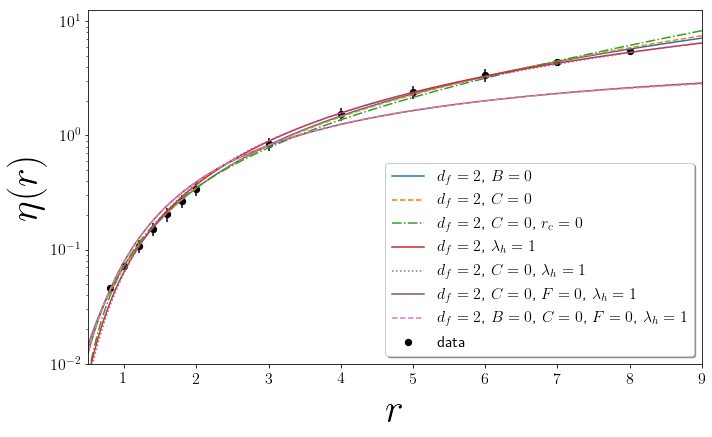
\includegraphics[width=0.5\textwidth]{eta_wellbehaved_comparison.png}
	\caption{Fit comparisons $\eta_{\textrm{alt}}(w)$, alternative transcritical form}
	\label{fig:etawellbehaved}
\end{figure}
%
\begin{table*}
	\begin{tabular}{|c|c|c|c|c|c|c|c|}
		\hline
		$r_s$ & $5.10 \pm 0.54$ & $5.05 \pm 0.36$ & $2.12 \pm 0.33$ & $1.81 \pm 0.08$ & $3.62 \pm 0.18$ & $6.57 \pm 0.39$ & $7.40 \pm 0.12$ \\
		$r_c$ & $-0.42 \pm 0.11$ & $-0.42 \pm 0.09$ & \textbf{0} & $ -0.15 \pm 0.07$ & $-0.29 \pm 0.09$ & $-0.62 \pm 0.10$ & $-0.70 \pm 0.03$ \\
		$\Sigma_s$ & $1.24 \pm 0.66$ & $-1.27 \pm 0.38$ & $13.16 \pm 5.72$ & $21.44 \pm 1.31$ & $3.19 \pm 0.45$ & $-0.67 \pm 0.32$ & $ 0.54 \pm 0.005$ \\
		$\eta_s$ & $3.16 \pm 0.11$ & $2.49 \pm 0.20$ & $0.56 \pm 0.40$ & $0.69 \pm 0.04$ & $2.48 \pm 0.09$ & $5.42 \pm 0.17$ & $6.08 \pm 0.82$ \\
		$d_f$ & \textbf{2} & \textbf{2} & \textbf{2} & \textbf{2}& \textbf{2} & \textbf{2} & \textbf{2} \\
		$\lambda_h$ & $0.44 \pm 0.04$ & $0.54 \pm 0.08$ & $0.70 \pm 0.05$ & \textbf{1} & \textbf{1} & \textbf{1} & \textbf{1} \\
		$B$ & \textbf{0} & $ -0.24 \pm 0.01$ & $-0.76 \pm 0.14$ & $-1.70 \pm 0.16$  & $-0.56 \pm 0.05$ & $-0.13 \pm 0.01$ & \textbf{0} \\
		$C$ & $0.46 \pm 0.10$ & \textbf{0} & \textbf{0} & $-0.31 \pm 0.04$ & \textbf{0} & \textbf{0} & \textbf{0} \\
		$F$ & $1.72 \pm 0.08$ & $1.22 \pm 0.16$ & $0.45 \pm 0.04$ & $-0.031 \pm 0.038$ & $0.35 \pm 0.03$ & \textbf{0} & \textbf{0}\\
		\hline
	\end{tabular}
	\caption{\label{tab:wellbehavedcompare} Table of the best fit values corresponding to Figures~\ref{fig:Sigmawellbehaved} and~\ref{fig:etawellbehaved}. Values in bold correspond to values fixed in the fit.}
\end{table*}

\bibliography{RFIM2D}{}

\end{document}
